\documentclass[11pt,letterpaper,oneside, titlepage]{scrartcl}
\usepackage{amsmath}
\usepackage{fancyhdr}
\usepackage{graphicx}

\usepackage[margin=1in]{geometry}

\usepackage{color}
\usepackage{listings}
\lstset{ %
language=C,                % choose the language of the code
basicstyle=\footnotesize,       % the size of the fonts that are used for the code
numbers=left,                   % where to put the line-numbers
numberstyle=\footnotesize,      % the size of the fonts that are used for the line-numbers
stepnumber=1,                   % the step between two line-numbers. If it is 1 each line will be numbered
numbersep=5pt,                  % how far the line-numbers are from the code
backgroundcolor=\color{white},  % choose the background color. You must add \usepackage{color}
showspaces=false,               % show spaces adding particular underscores
showstringspaces=false,         % underline spaces within strings
showtabs=false,                 % show tabs within strings adding particular underscores
frame=single,           % adds a frame around the code
tabsize=2,          % sets default tabsize to 2 spaces
captionpos=b,           % sets the caption-position to bottom
breaklines=true,        % sets automatic line breaking
breakatwhitespace=false,    % sets if automatic breaks should only happen at whitespace
escapeinside={\%*}{*)}          % if you want to add a comment within your code
}


\pagestyle{fancy}
\fancyfoot{}
\fancyhead{}
\fancyfoot[CE,CO]{\thepage}
\fancyhead[LO,LE]{Detecting Texts Copied from a Common Source\\ Toth, Kiffer, Fein, Sheriff}

% disables chapter, section and subsection numbering
\setcounter{secnumdepth}{-1} 

\begin{document}
\title{Detecting Texts Copied from a Common Source}
\subtitle{CS 4780 Final Project Team 11}
\date{\today}
\author{Will Kiffer - wjk56\\Jeremy Fein - jdf226\\Kimberly Sheriff - kgs45\\Brian Toth - bdt25}
\maketitle


\tableofcontents
\clearpage

\section{Introduction}

The internet is filled with computer generated spam content meant to game search engine results, product reviews, and spam e-mail detectors. Search engine optimization (SEO) and other spamming companies sell services to flood websites with fake content in order to falsely promote their customers. To create lots of fake content that appears to be uniquely written, companies can pay a human to write a single, unique article and then use techniques to transform, or “spin”, this article into millions of syntactically distinct but semantically identical articles. Although these articles may appear unique, they are actually inherently plagiarized. These millions of distinct articles are then posted automatically on blogs and review sites to promote or hyperlink to the SEO company’s client. If the web services could detect when two pieces of content are similar, it could be deduced that they came from a common source and therefore is spam content.

In this paper we discuss novel methods of identifying if two articles are generated from a common source. By exploiting the methodology of the spam and SEO companies, we aim to outperform simple methods such as cosine similarity. With a dataset of “article formulas” that can be used to generate millions of articles, learning can be done to predict if two articles are unique or plagiarized. Two methods, a discriminative analysis with SVM and generative modeling using HMM, are proposed, both of which perform better than simple cosine similarity. These methods could be deployed in a large scale spam detection service.

\section{Problem Definition and Methods}

\subsection{Task Definition}

Formally, our task is given a pair of articles A1 and A2, determine whether or not they are derived from a common source, or in other words if they are duplicate content. Articles A1 and A2 are considered derived from a common source article B if both A1 and A2 are semantically identical to B. This can be achieved by algorithmically replacing words in B with unique contextual synonyms to create A1 and A2. SEO and spam companies would pay to write the source article B, then algorithmically modify B to create millions of articles like A1 and A2. If it could be predicted that two articles A1 and A2 were generated from the unknown article B, then the spam content can be detected preemptively.

To accomplish this task we are using a manually processed database of articles obtained from a major SEO company. These articles are of the form: "I {like|love} the {small|little|medium-sized} {dogs|canines}". A sample source article is included in Appendix A. From now on we will refer to a single group of contextually similar words/phrases such as {like|love|adore} as a "spin group" and as individual members such as like, love, adore as the spin group's members or elements. We will also refer to articles containing these spin groups as "source articles". An actual article can be generated by selecting one spin group element from each spin group. Appendix B shows two example generated articles from the source article in Appendix A.

Our dataset contains 2959 source articles. Each source article has on average 215.15 spin groups. Each spin group has on average 3.75 members. This means that each source article could potentially generate 3.75215.15 unique articles. These unique articles are correct both semantically and syntactically. They make sense. They are actual articles that you may find on the internet – particularly on scam blog networks. Some of them may not be the best written or most insightful articles, but they make sense and have meaning.  While that is a huge amount of unique articles, many of these unique articles are extremely similar. Some of them differ by only one word, others only by a couple.

The goal of this project is to create a similarity measure that, given two articles, will produce a number representing the articles semantic similarity. This number can be used in a binary classifier to classify if the two articles are indeed from the same source or not. Using our dataset, we can generate numerous positive examples (two articles that are from a common source) and negative examples (two articles not from a common source), determine the similarity number for each example, and produce an ROC curve to show the effectiveness of our binary classifier. Our learned similarity measure should do better than a binary classifier using simple cosine similarity.

Each source article is also annotated with keywords describing each article. These keywords are useful for generating pairs of articles that are not duplicates, yet are still about the same topic. These pairs can be used as negative examples from our classifier. Without these keywords all our negative examples would be extremely dissimilar from the start just by virtue of being about different topics.

\subsection{Baseline}

The simplest baseline measure that we will use is cosine similarity between the two documents word vectors, where the word vectors are created using the bag of words model. Our classifier simply computes the cosine similarity between two documents and classifies them as duplicates if the similarity is above a certain threshold. We computed the cosine similarity for 1000 positive examples (pairs of duplicate articles) and 1000 negative examples (pairs of unique articles with the same keywords). We then computed the true positive rate and the false positive rate while varying the threshold value. Plotting these values we obtained the following ROC curve.

\begin{figure}[h!]
  \centering
  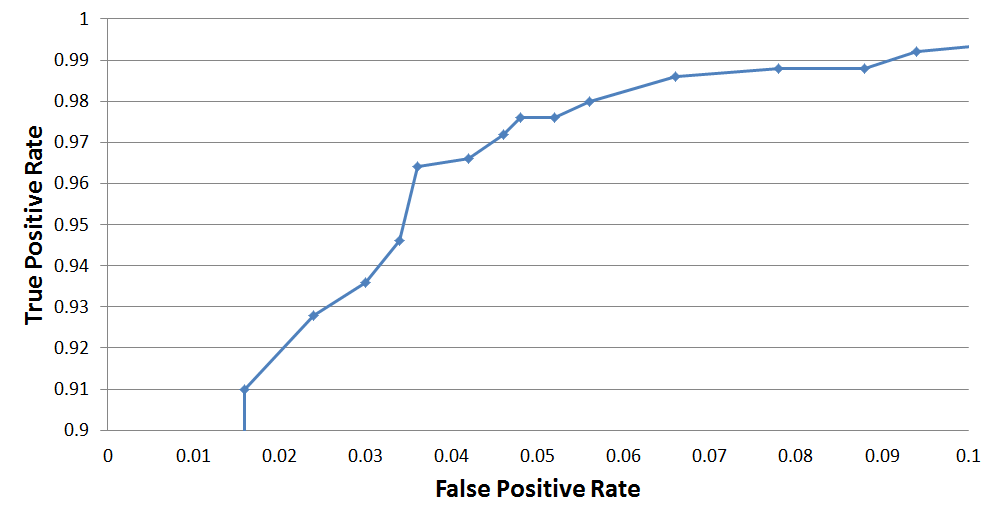
\includegraphics[width=1\textwidth]{baseline_ROC}
  \caption{Baseline ROC Curve}
  \label{fig:baseline_ROC}
\end{figure}

\clearpage

At it’s best, cosine similarity was able to achieve about a 96.5\% true positive rate and only about a 3.5\% false positive rate. 



\subsection{Algorithms and Methodology Overview}


\subsubsection{Data Preprocessing}

Our data set of source articles is in .xml format. For use, we parse the file into Python using the open source XMLToDict Python extension. Once in Python, it is simple to filter out blank or unusable source articles (those with bad formatting or limited keyword information) and provide ways to standardize the data. These standardizations include lemmatization of words, stemming of words, removing stop words, etc. Natural Language Toolkit (NLTK) and WordNet are used to achieve these tasks as shown in Figure ~\ref{fig:filtering}.

\begin{figure}[h!]
  \centering
  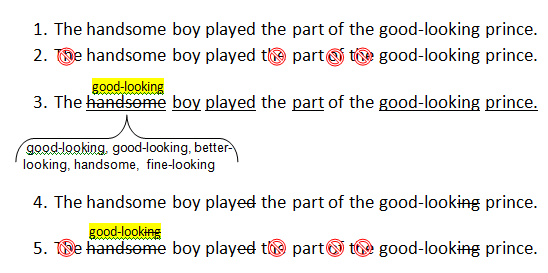
\includegraphics[width=0.75\textwidth]{filtering}
  \caption{Filtering Techniques}
  \label{fig:filtering}
\end{figure}

Figure ~\ref{fig:filtering} shows a sample sentence (line 1) with the three techniquest applied in isolation and together. Line 2 shows the effects of stop word removal. Line 3 shows synonym replacement where a word is replaced with its most common synonym. For example, if the words “like” “love” and “adore” all appeared in the data set, each instance of “like” “love” or “adore” would be replaced with “like.” In the example of line 2, NLTK and Wordnet were used to accomplish this task for each word in each article. First, the part of speech tagger in NLTK was used to denote the part of speech for the word "handsome", adjective Next, using the WordNet database, the synonyms for all senses of "handsome" the adjective were found and put into a list. Finally, this list of synonyms was sorted by order of occurence and the most common synonym replaced the word. Line 4 shows the stemming of words which takes a word and replaces it with the stem of the word. In this case, "played" becomes "play". Line 5 shows the combination of all three techniques with stemming occuring last.

In addition to filtering individual articles, we can also determine the types of articles to be used in our trianing and test sets. Since each article is denoted by a set of keywords, we can choose to use only articles that share every keyword, at least one keyword, or give no restrictions on keyword similarity.

To insure that we are using similar training and test sets for all methods, we decided to train on odd numbered source articles and test on even numbered source articles.
%TODO:
%<TALK ABOUT TRAINING AND TEST SETS (even and odd)>


\subsubsection{SVM Approach}

This supervised learning approach uses a soft margin support vector machine (SVM) to classify articles. The source articles are labeled with a unique number and this number is also given to every spun article that comes from that source. For each source article, the spun articles are relabeled as +1 if the article comes from that source or -1 if the article does not come from that source. The features for the SVM are all of the words in the English language. We used bag of words to create the feature vector for each spun article. Binary classifications are made for each source article using svmlite.

This method has the potential to be very useful because it does not require specific knowledge about the form of the source articles.

We hypothesize that, given two articles A1 and A3, this model can be used to determine if A1 and A2 came from the same article by running both articles through the SVM. If the two articles are from the source, the SVM should output the same source for both articles.

%TODO:

\subsubsection{HMM Approach}

Our generative approach aims to use a hidden markov model (HMM) to predict a hidden source article that could have generated an actual article. The intuition is that a sentence in an actual article can be modeled as a sequence of phrases that was emitted from a hidden sequence of spin groups. Each spin group in our known source articles can be modeled as a hidden state; a single hidden spin group state has equal chance to emit any of its elements. Transitions between hidden spin group states are drawn from the sequences of spin groups in the known source articles. With these transition and emission probabilities, a modified viterbi algorithm can predict a sequence of spin groups from an article. We hypothesize that this sequence of spin groups is essentially the result of adding in possible contextual synonyms to the article - just as is done when a human writes a source article from a unique one.

Moving forward with this approach, a primary initial concern is the running time of the Viterbi algorithm. Many of our decisions will be motivated by the desire to keep the running time as low as possible, which is mainly influenced by the number of hidden states (number of unique spin groups).

We hypothesize that, given two articles A1 and A2, this generative model can be used on A1 to predict a potential source article S1 that is semantically likely to have generated A1. Then, if A1 and A2 were actually from a common source, S1 would also be able to semantically generate A2.


\section{Experimental (and/or Theoretical) Evaluation }



\subsection{SVM Methodology}

%What are the criteria you are using to evaluate? How does this evaluation (e.g. experiment) relate to the questions you are trying to answer? Describe the experimental methodology that you used. What is the training/test data that was used, and why is it realistic or interesting? Exactly what performance data did you collect and how are you presenting and analyzing it? Comparisons to competing methods that address the same problem or to variations of your own algorithm are particularly useful. Give enough detail about your experiment setup so that others could reproduce the work.
%TODO
%<SVM METHODOLOGY AND EVALUATION CRITERIA HERE>




\subsection{SVM Results}

%Present the quantitative results of your experiments. Graphical data presentation such as graphs and histograms are frequently better than tables. Explain the basic findings by explaining the results contained in the tables and graphs.

The results of SVM showed that filtering does improve accuracy in learning as shown in Figure ~\ref{fig:svm}. The baseline gives SVM accuracy of 66\%, but the SVM has 100\% when all filtering methods are used. The filtering techniques in rough order of efficacy are: stopwords removed, replaced synonyms, standardized articles. Standardized articles refers to stemming and lemitizing the articles. Figure ~\ref{fig:svm} shows the results for the case where the articles share every keyword.


\begin{figure}[h!]
  \centering
  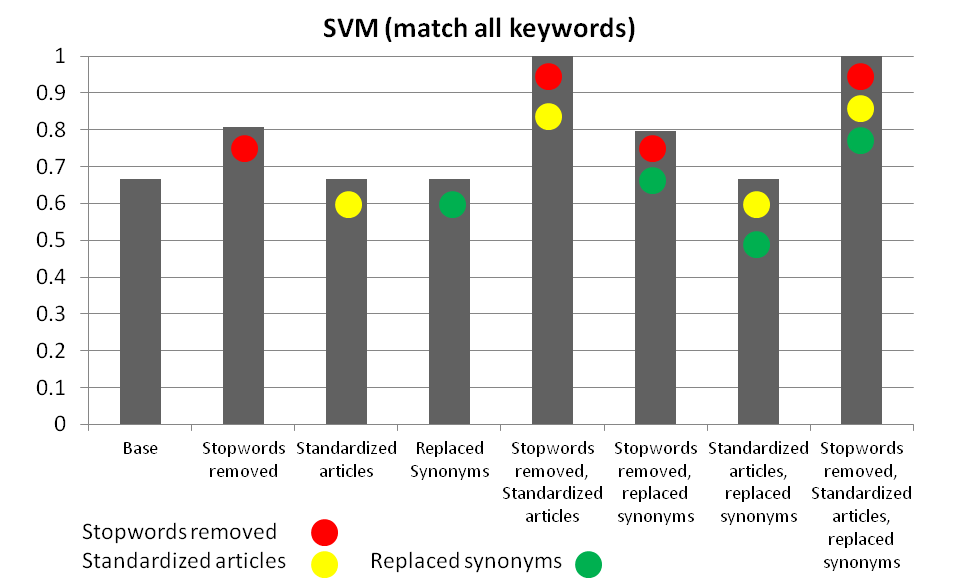
\includegraphics[width=0.75\textwidth]{svm_allmatches}
  \caption{SVM Results Histogram}
  \label{fig:svm}
\end{figure}

\clearpage

\subsection{HMM Methodology}

To create a working HMM model, we first need to model all source articles as sequences of spin groups. Words in source articles that are not members of spin groups are treated as a spin group with one element of that word. For example “I {like|love} the {dog|canine},” transforms into the spin groups “{I}, {like|love}, {the}, {dog|canine}”.

Our HMM is designed to classify a single sentence. Therefore to classify an article, we classify each sentence individually. We chose to classify sentences at a time for two reasons. First, transitioning between the last spin group of a sentence and the first spin group of the next sentence doesn’t make much sense. Intuitively, the word that starts a sentence has little to do with the word that ended the last sentence. Additionally, if our HMM classified articles as a whole, the start probabilities would be which spin groups are most likely to start an article. Again, this seems to make less sense than the alternative of classifying a single sentence, where the start probabilities would be which spin groups are most likely to start a sentence. Finally, it would be easy for a computer to add more variability to generated spam articles by switching sentence order; by treating each sentence individually, this trick should not matter in our final classification.

\subsubsection{Clustering}

Our dataset contains over 150,000 unique spin groups. Running viterbi on this large of a state space is simply unfeasible, so we need to reduce the number of spin groups. The most obvious way to reduce the number of spin groups is to use spin groups seen in a random subset of the source articles. While this approach is effective at reducing the number of spin groups and is easy to implement, it is not ideal since we lose information by just taking a random subset.

A better approach is to use a clustering method to reduce the number of spin group states. This has the added benefit of smoothing some of the noise in the dataset, where unique spin groups only differ by a single word. However, we have to be very careful when we attempt this clustering so that we don’t accidently combine two spin groups that are actually semantically different and therefore lose information.

Because of this, we chose to use HAC clustering with complete-link similarity. Similarity between two spin groups was computed as the number of elements the spin groups have in common divided by the total number of elements in both spin groups. Complete-link was used to ensure that all members of a cluster were similar to every other member.

However even clustering was unfeasible on 150,000 spin groups. We therefore only used spin groups from 250 random training articles which turned out to be around 25,000. We then clustered these spin groups into about 13,000 spin group clusters. These spin group clusters are the hidden states.

\subsubsection{Transition probability estimation}

Although we were only able to use spin groups gathered from 250 training articles, we could use the entire training set to estimate transition probabilities between spin group clusters. To do this, we keep track of the set of unique spin groups as well as a mapping from each spin group to the cluster of spin groups that it belongs to. Then, for each sentence in each source article in our training set, we look at every bigram of spin groups. We map the spin groups in the bigram to clusters, and keep track of the number of times a unique cluster occurs in our training set. If both spin groups map to clusters (meaning we have seen both spin groups in the original 250 random training articles the spin group clusters were derived from), then we increase the number of times the first spin group cluster can transition to the second spin group cluster. Using these bigram counts, we can calculate the transition probability between two spin group clusters.

Since we have not seen every possible bigram in our training data, many unseen bigrams will have a 0\% probability of occurring. To fix this, we introduce Witten-Bell smoothing, where the probability of an unseen bigram occurring will be estimated by the unigram probabilities of the spin group clusters and the number of times those spin groups are involved in bigrams in general. This allows our HMM to sometimes predict untrained transitions that may ultimately lead to a more semantic spin group prediction.

\subsubsection{Emission probability estimation}

The probability that a given spin group cluster will emit a given phrase is the chance that, if an element were to be picked at random from the spin group cluster, it will be the given phrase. If the phrase is part of the spin group cluster, this will be exactly 1 divided by the number of elements in the spin group. If not, then this is exactly 0.

\subsubsection{Modified Viterbi}

Our implementation of Viterbi was straightforward except for one part. Since spin group elements could be variable length (such as “{like|really like}”) this meant that one hidden spin group state could potentially generate more than one output state. To do this, we modified viterbi so that a state was a tuple of (Spin group, Number of output states it generated). From analyzing our dataset, we found that over 99\% of spin groups had no elements longer than 4 words. We therefore allowed the number of output states a spin group generated vary from 1-4, and effectively quadrupled our state space. 

We also created an additional special hidden state for unknown words. If we have never encountered a word before, then the emission probability for every state will be 0, and therefore we just assign it to the unknown state. Below is a diagram illustrating how this modified Viterbi algorithm worked.

\begin{figure}[h!]
  \centering
  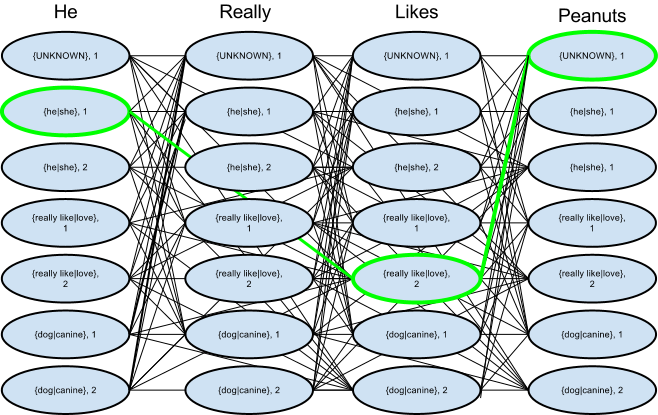
\includegraphics[width=1\textwidth]{hmm_spin_group}
  \caption{HMM Spin Group}
  \label{fig:hmm_spin_group}
\end{figure}

\clearpage

In the above example the hidden spin group {really like|love} generated the two output states ‘really like’, and since we have never seen the word ‘peanut’ before, it is assigned the unknown spin group.

\subsubsection{Evaluation}

With a working HMM model to predict the most likely sequence of spin groups that could have generated a given article, we can then experimentally test our hypothesis stated in 2.3.3. Again, our hypothesis is that given articles A1 and A2, we can make spin group predictions S1 and S2; if potential common source S1 is equally likely to generate A1 and A2, and other potential common source S2 is equally likely to generate A2 and A1, then it is likely A1 and A2 are from the same common source. Since some words in A2 will not be present in S1, there would be a 0\% chance that S1 would emit A2; thus, we need a better measure to show if S1 (or S2) could equally generate A1 and A2. Instead, it is thought that if S1 can generate A1 and A2 equally, then the cosine similarity between S1 and A1 should be similar to the cosine similarity between S1 and A2. The ratio of these cosine similarities would tell us how similar they are - if the similarities are the same, the ratio will be 1, and if they are disparate it will be less than 1 (A2 will never be more similar than A1). Cosine similarity is done on word count vectors of the words in spin groups and in the articles. We can then average the cosine similarity ratios for S1 and S2 to produce an overall similarity measure for A1 and A2:

$Similarity(A1, A2) = AVG\{ cos(A2, S1)cos(A1, S1) , cost(A1, S2)cos(A2, S2) \}$

This measure can then be placed in a binary classifier with varying thresholds to make an ROC graph to rate the effectiveness of the similarity measure in a binary classifier. The HMM is trained on even numbered source articles, and positive/negative examples are drawn from only odd numbered source articles. Remember, negative examples (two articles not from a common source) are chosen to have the same keywords and thus be about the same topic.

\subsection{HMM Results}

%TODO
wtf


\subsection{Discussion}

%TODO How do the results answer your questions? What conclusions do the results support about the strengths and weaknesses of your method compared to other methods? How can the results be explained in terms of the underlying properties of the algorithm and/or the data. 

\section{Related Work}

Can you say anything about related work from your background readings? It may be possible to answer the following questions for each piece of related work that addresses the same or a similar problem. What is their problem and method? How is your problem and method different? Why is your problem and method better? 

\section{Future Work}
\begin{itemize}

\item Use thresholding to allow for "none of the above" classification.  This would prevent a sufficiently dissimilar article from accidentally being marked as coming from the same source as another.

\item Consider training on examples that are classified only as "same source" or "not same source".  This would attempt to learn common words that are used by the authors of spin groups.

\item Explore using K-Mean clustering to produce K spin group clusters. Will allow to train on all data while keeping number of hidden states small.

\item Use our data to better estimate unigram probabilities for improved transition and emission smoothing.

\item Match unseen spin groups to most similar cluster to better estimate transition probabilities.

\end{itemize}
%TODO What are the major shortcomings of your current method? For each shortcoming, propose additions or enhancements that would help overcome it.


\section{Conclusion}

Briefly summarize the important results and conclusions presented in the paper. What are the most important points illustrated by your work? How will your results improve future research and applications in the area?

\section{Appendices}

\subsection{Appendix A: Snippet of Sample Source Article}

\begin{verbatim}{Whenever|When|At any time when|When you are|Whenever you are|Should you be|If you're|
If you happen to be|If in case you're} {planning|preparing|organizing|setting up} 
{weddings|wedding ceremonies|marriage ceremonies|wedding events}, the groom {and the|
and also the|plus the} {bride|bride-to-be|new bride} {need to|have to|really need to|
will need to} {think about|consider|take into consideration|contemplate} {everything|
every thing|almost everything} {in order to|as a way to|so that you can|to be able to}
{please|satisfy|gratify|entertain} {all the|all of the|every one of the|each of the}
{people|individuals|men and women} {attending|visiting}. {One of the|Among the|
One of several|One of the several} {problems|issues|troubles|complications} that 
{usually|generally|typically|commonly} {appears|shows up|arises|comes up} is what 
{souvenirs|mementos|gifts} to be {used|utilized|employed}. {Most of them|Many of them|
A lot of them|Some of them} are {designed|created|developed|made} for female {guests|
visitors|attendees} {and not|rather than|instead of} for the men. {Because|
Simply because|Due to the fact} of this, it {might|may|could} be a {great|fantastic|
good} {idea|concept|notion|strategy|plan} {to use|to make use of|to implement} koozies
for wedding favors, {as they|because they|since they} are {perfect|ideal|best} for 
{male|men|guys} {guests|visitors|attendees}.
\end{verbatim}
 
\subsection{Appendix B: Two Resulting spun article from Appendix A}


Should you be preparing weddings, the groom and the bridetobe will need to think about everything in order to satisfy all of the individuals attending. One of several issues that commonly appears is what gifts to be employed. Many of them are created for female attendees instead of for the men. Simply because of this, it might be a fantastic idea to use koozies for wedding favors since they are perfect for male attendees.

 
Whenever organizing wedding events, the groom and also the bride have to take into consideration almost everything as a way to please every one of the people visiting. One of the several problems that usually shows up is what souvenirs to be used. Some of them are made for female visitors and not for the men. Because of this, it could be a great concept to implement koozies for wedding favors, because they are ideal for guys visitors.




\clearpage

\subsection{Code}

\begin{lstlisting}

\end{lstlisting}

\end{document}
